\section{Architektura IoT sítí}
  V blízké době se očekává stále větší nárůst zařízení, která jsou připojena k internetu.
  Dle odhadů by jejich počet měl v roce 2020 překročit 30 miliard \cite{iotDevices}.
  Pro takové množtví připojení už není možné, aby každé zařízení komunikovalo přímo
  se vzdáleným datovým centrem, protože nároky na potřebnou šířku pásma by byly 
  obrovské \cite{fog}.
  Dalším problémem je často velmi omezený výkon připojených prvků, který je nezbytný pro 
  použití bezpečnostních funkcí umožňujících kompletně zabezpezpečenou komunikaci. 
  
  Řešení těchto problémů je do probíhající komunikace přidat několik podvrstev, 
  které umožní přesunout výpočetní výkon blíže ke koncovým zařízením, a tím celý
  proces zpracování dat provést efektivněji.
 \subsection{Fog computing} 
 Fog computing je rozšíření Cloud computingu, které spočívá v přesunutí výpočetního
 výkonu blíže k okraji sítě. Rozšíření je umožněno pomocí přidání síťových zařízení,
 které kromě síťových funkcionalit nabízí i výpočetní výkon pro běh programů. Programy 
 je často možné nasadit pomocí konterjnerů nebo samostatných virtuálních strojů, což 
 velmi usnadňuje jejich distribuci \cite{fog}.
 
 Porovnání klasické a Fog architektury se nachází na obrázku \ref{obr.fog}. V reálném nasazení může
 být použito i více Fog vrstev, kde každá provádí určitý stupeň předzpracování a řízení
 dat.
\begin{figure}[ht]
\begin{center}
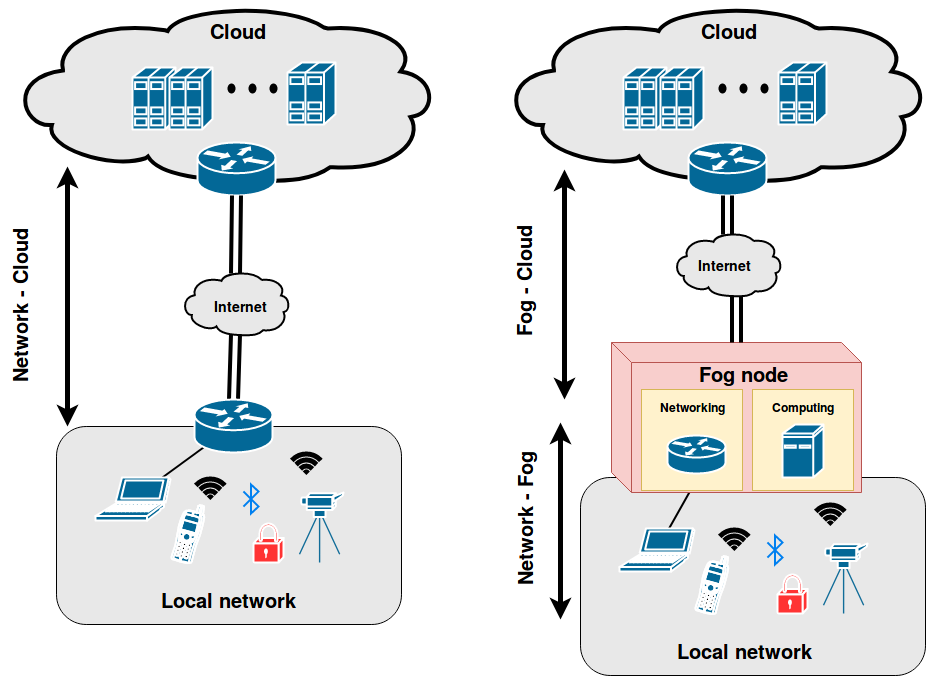
\includegraphics[scale=0.38]{pictures/fog}
\caption{Porovnání klasické a fog architektury}
\label{obr.fog}
\end{center}
\end{figure}
 Zavedením principů Fog computingu vznikají pro síť následující výhody:
 \begin{itemize}
 \item \textbf{Zlepšení bezpečnosti}
 
     Fog nodes jsou trvale napájené a připojené k internetu. Podporují pokročilé
     bezpečnostní funkce, a proto je možné například vytvářet šifrované tunelové
     spojení pro chráněný přenos dat.
 \end{itemize} 
 
 \subsection{IoT brána} 
 \subsection{Komunikační model}
 \subsection{Bezpečnostní hrozby komunikačního modelu}
 \section{Analýza síťových protokolů}
 % popis funkce fungování MQTT, COAP, (AMQP)
 \section{Analýza senzorových protokolů}
 % popis a bezpečnostní analýza ZWave a Bluetooth
 \section{BeeeOn brána}
 \section{NEMEA framework}
 \section{Existující řešení}
 % aktuální řešení funguje na cetrálním monitorovacím prvku, které monitoruje IP
 % teprve nedávno vznikly signatury pro SCADA
 \section{Analýza požadavků}
 \section{Zvolené řešení}
